\section{Datenspeicherung}
\label{chap:data}
Die Datenspeicherung beinhaltet die gespeicherten Messwerte der Sensoren. Die Daten werden dann in einem *.txt-File nicht flüchtig gespeichert. Bei Beschädigung der Hardware können dann die zuletzt erfassten Daten immer noch mittels eines SD-Karten-Adapters von einem Computer ausgelesen werden. Als Kommunikationsprotokoll für das Schreiben und Auslesen der Karte wird SPI verwendet.\\
%\subsection{Breakoutboard}
%Das Breakoutboard (siehe Abb. \ref{fig:muSDBreakout}) kann wegen des intern implementierten \textit{CD74HC4050 high-speed logic level translators}\footnote{konvertiert eine high-level logik in eine low-level logik} mit 5V betrieben werden. Das Arduino Mega Board und das Breakoutboard werden über SPI (siehe Kapitel \ref{subsubsec:spi}) nach dem Master-Slave Kommunikationsprinzip miteinander verbunden. 
%\begin{figure}[h]
%\centering
%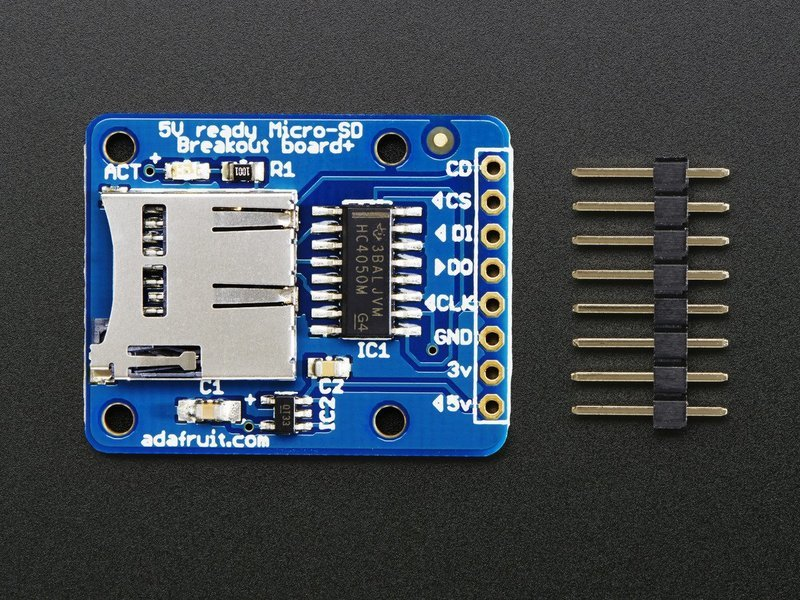
\includegraphics[width=0.5\linewidth]{graphics/Datenspeicherung/micro_sd_card_breakout.png}
%\caption{254 $\mu$SD-Breakoutboard von Adafruit \cite{ladyada2018}}
%\label{fig:muSDBreakout}
%\end{figure}

%\subsubsection*{Verdrahtung}
%SD-Karten erfordern viel Datenübertragung. Deshalb kann die beste Leistung erbracht werden, wenn sie an die Hardware-SPI-Pins eines Mikrocontrollers angeschlossen werden. Dabei wird es wie folgt miteinander verbunden: \cite{ladyada2018}
%\todo[inline]{Hier vielleicht noch das Schema hinzufügen wie es Hardwaremässig implementiert wird.}
%\begin{itemize}
%\item \textbf{5V} und \textbf{GND} Pins jeweils auf die \textbf{5V} und \textbf{GND} Pins des Arduino Mega Boards
%\item \textbf{CLK} auf die Pinnummer \textbf{52}
%\item \textbf{DO} auf die Pinnummer \textbf{50}
%\item \textbf{DI} auf die Pinnummer \textbf{51}
%\item \textbf{CS} auf die Pinnummer \textbf{53}
%\end{itemize}
%\newpage

\subsection{$\mu$SD-Karte}
\begin{minipage}{0.44\textwidth}
\centering
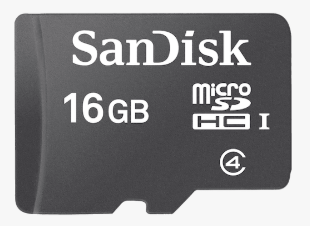
\includegraphics[width=0.4\textwidth]{graphics/Datenspeicherung/micro_sd_card_16GB.png}
\captionof{figure}{16 GB $\mu$SD-Karte \cite{musdkarte}}
\label{fig:muSDKarte}
\end{minipage}
\begin{minipage}{0.55\textwidth}
Bei der $\mu$SD-Karte muss auf die Kompatibilität mit dem Breakoutboard geachtet werden. Dafür sind folgende Kriterien zu beachten:\\
\begin{itemize}
\item Die $\mu$SD-Karte muss FAT16 oder FAT 32 formatiert sein.
\item Es sind nur die SD und SD High Capacity (SDHC) kompatibel.\\
\end{itemize}
\end{minipage}
Für die Umsetzung dieses Projektes wurde eine $\mu$SD-Karte der SD-Familie SDHC \Romannum{1} verwendet (siehe Abb. \ref{fig:muSDKarte}). SDHC sind Kapazitäten bis zu 32GB möglich und FAT32 formatiert. \cite{muSDspez}\\ %\todo[inline]{Es könnte noch auf die Anschlüsse der $\mu$SD-Karte eingegangen werden. Gäbe aber nur Sinn wenn ein Print erstellt werden muss wo das Breakoutboar nachkonstruiert wird.}

Die Grösse eines Strings lässt sich nach der Gleichung \ref{equ:berechnung_stringgroesse} berechnen, wenn angenommen wird, dass jeder Buchstaben (char) 8 Bit hat und zum Schluss noch ein Terminator für das Stringende angehängt wird:

\begin{equation}
\centering
Anzahl\ Zeichen * 1\ Byte + 1 = String\ Grösse\ in\ Byte
\label{equ:berechnung_stringgroesse}
\end{equation}

Bei einer Speicherung der Daten nach der Struktur in Abb. \ref{fig:datenausgabe} würden somit leicht aufgerundet ca. 216 Byte pro Speichersatz benötigt werden.\\

Da momentan eine 16GB grosse $\mu$SD-Karte verwendet wird, ergeben sich daraus

\begin{equation}
\dfrac{16E9}{216}=74.1E6 \approx \underline{\underline{74E6}}
\end{equation}

Speichersätze. Würden in einem zehn Minuten Zeitintervall ein Speichersatz abgespeichert werden, dann könnten 1411 Jahre 40 Wochen 4 Tage 21 Stunden 20 Minuten lang Werte von der Wetterstation abgespeichert werden. Diese Anzahl könnte noch verdoppelt werden, da wie oben bereits erwähnt $\mu$SD-Karten bis zu 32GB kompatibel sind.\\

\newpage

\subsection{Implementation in die Firmware}
Für die Implementation in die Firmware, um mit dem Breakoutboard über SPI zu kommunizieren und die $\mu$SD-Karte zu beschreiben, resp. zu lesen, wurden direkt die bereits existierenden Librarys <SPI.h>\footnote{ <*.h> bezieht sich auf ein include-Verzeichnis unter dem Compiler-Installationsverzeichnis} und <SD.h> von Arduino inkludiert. In der Arduino IDE können bereits vorgefertigte Expample-Codes (siehe Abb. \ref{fig:exampleCodes}) zur weiteren Interpretation, wie mit diesen Librarys $\mu$SD-Karten gelesen und geschrieben werden können, verwendet werden.\\
\begin{figure}[h]
\centering
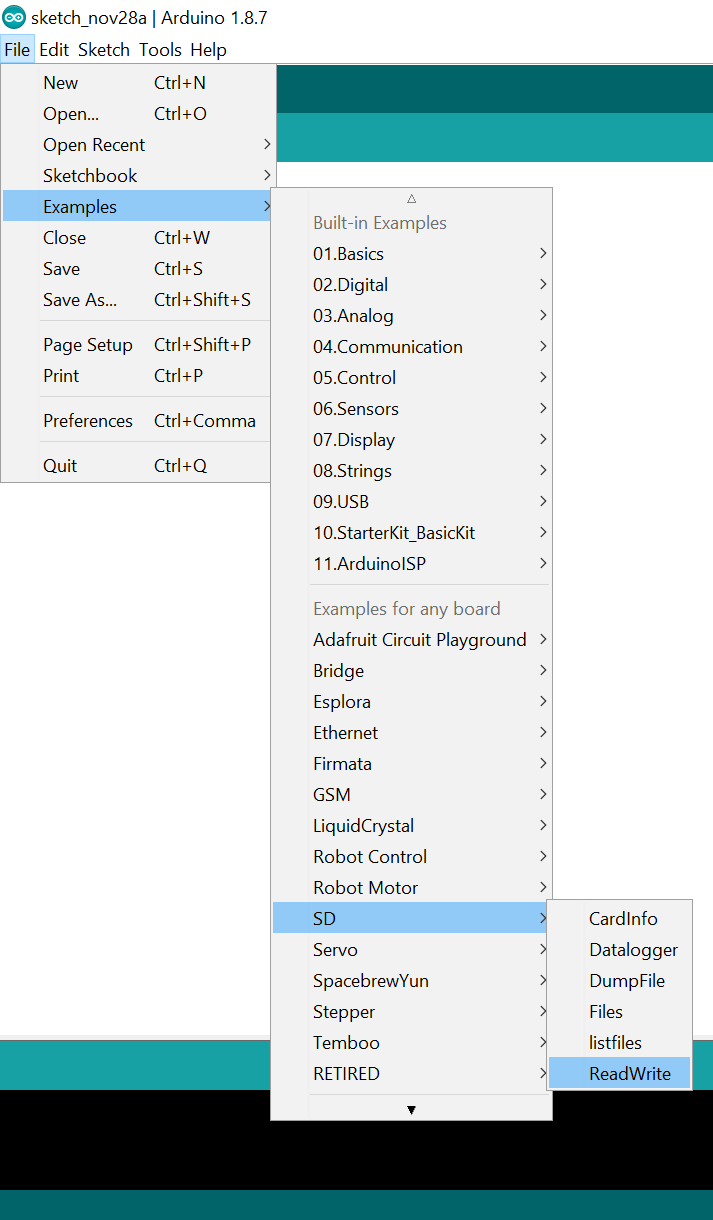
\includegraphics[width=0.48\textwidth]{graphics/Datenspeicherung/read_write_examples.PNG}
\caption{Example-Codes der Arduino IDE zum Lesen und Schreiben von SD-Karten.}
\label{fig:exampleCodes}
\end{figure}

Für eine übersichtlichere Programmstruktur und einfachere Handhabung wurden die Exampel-Codes für die korrekte Implementation angepasst und in Funktionen verpackt. Die Funktionen sind extern im Headerfile ''SDCard.h''\footnote{ ''*.h'' bezieht sich relativ auf das aktive Projektverzeichnis} deklariert und im SDCard.cpp initialisiert.
\begin{itemize}
\item \textcolor{blue}{void} \textcolor{orange}{getCardInformations}()
\item \textcolor{blue}{void} \textcolor{orange}{readFileSDCard}(\textcolor{Dandelion}{String} filename)
\item \textcolor{blue}{void} \textcolor{orange}{writeFileSDCard}(\textcolor{blue}{double} value2save, \textcolor{Dandelion}{String} filename)
\item \textcolor{blue}{void} \textcolor{orange}{deleteFileSDCard}(\textcolor{Dandelion}{String} filename)
\end{itemize}
%\todo[inline]{Funktionen könnten noch beschrieben werden. Noch Abklären, ob die Fußzeilen nötig sind!}